%latex model.tex
%bibtex model
%latex model.tex
%latex model.tex
%pdflatex model.tex

%se poate lucra si online (de ex www.overleaf.com)


\documentclass[runningheads,a4paper,11pt]{report}

\usepackage{algorithmic}
\usepackage{algorithm} 
\usepackage{array}
\usepackage{amsmath}
\usepackage{amsfonts}
\usepackage{amssymb}
\usepackage{amsthm}
\usepackage{caption}
\usepackage{comment} 
\usepackage{epsfig} 
\usepackage{fancyhdr}
\usepackage[T1]{fontenc}
\usepackage{geometry} 
\usepackage{graphicx}
\usepackage[colorlinks]{hyperref} 
\usepackage[latin1]{inputenc}
\usepackage{multicol}
\usepackage{multirow} 
\usepackage{rotating}
\usepackage{setspace}
\usepackage{subfigure}
\usepackage{url}
\usepackage{verbatim}
\usepackage{xcolor}
\usepackage{textcomp, gensymb}
\usepackage{caption}
\usepackage{combelow}

\usepackage{array,amsfonts}

\newcommand\myfunc[5]{%
  \begingroup
  \setlength\arraycolsep{0pt}
  #1\colon\begin{array}[t]{c >{{}}c<{{}} c}
             #2 & \to & #3 \\ \\
          \end{array}%
  \endgroup}

\geometry{a4paper,top=3cm,left=2cm,right=2cm,bottom=3cm}
\definecolor{forestgreen}{RGB}{52,194,48}
\definecolor{mycolor}{RGB}{0, 153, 255}

\pagestyle{fancy}
\setlength{\headheight}{23.11996pt}
\addtolength{\topmargin}{-11.11996pt}
\fancyhead[R]{An Analysis of Multitask Models for Histopathology}
\fancyhead[L]{Data Mining Research Report}


\renewcommand{\headrulewidth}{2pt}
\renewcommand{\footrulewidth}{1pt}
\renewcommand{\headrule}{\hbox to\headwidth{%
  \color{mycolor}\leaders\hrule height \headrulewidth\hfill}}
\renewcommand{\footrule}{\hbox to\headwidth{%
  \color{mycolor}\leaders\hrule height \footrulewidth\hfill}}

\hypersetup{
pdftitle={artTitle},
pdfauthor={name},
pdfkeywords={pdf, latex, tex, ps2pdf, dvipdfm, pdflatex},
bookmarksnumbered,
pdfstartview={FitH},
urlcolor=cyan,
colorlinks=true,
linkcolor=black,
citecolor=red,
}
% \pagestyle{plain}

\setcounter{secnumdepth}{3}
\setcounter{tocdepth}{3}

\linespread{1}

% \pagestyle{myheadings}

\makeindex


\begin{document}
\nocite{*}
\begin{titlepage}
\sloppy

\begin{center}
BABE\c S BOLYAI UNIVERSITY, CLUJ NAPOCA, ROM\^ ANIA

FACULTY OF MATHEMATICS AND COMPUTER SCIENCE

\vspace{6cm}

\Huge \textbf{An Analysis of Multitask Models for Histopathology}

\vspace{1cm}

\normalsize Data Mining Research Report

\end{center}


\vspace{4cm}

\begin{flushright}
\Large{\textbf{Student}}\\
Alexandru Manole
\end{flushright}

\begin{flushright}
\Large{\textbf{PhD Scientific Coordinator}}\\
Prof. Dr. Laura Dio\c{s}an
\end{flushright}

\begin{flushright}
\Large{\textbf{Course Coordinator}}\\
Prof. Dr. Anca Andreica
\end{flushright}


\vspace{3cm}

\begin{center}
2023-2024
\end{center}

\end{titlepage}

\pagenumbering{gobble}

\begin{abstract}
Artificial Intelligence has the potential to streamline and facilitate numerous processes in the medical field, increasing the quality of life for millions and potentially saving lives. One area which requires a lot of effort when it comes to diagnosing severe diseases like cancer is Histopathology. Recently, a modern learning strategy, Multi-task learning, was applied in Digital Histopathology in order to obtain relevant medical information from histological images. This paradigm is able to increase performance by learning multiple objectives simultaneously resulting in more general features. The resulting methods reduces overfitting and training times while increasing data efficiency making it a suitable choice for the high-dimensionality low sample size sets from the medical field. The aim of this report is to present novel multi-task approaches with applications in Histopathology, analyse them, showcase their advantages and drawbacks and identify possible future research directions.
\end{abstract}


\tableofcontents

\newpage

\listoffigures

\newpage

\setstretch{1.5}

\newpage

\pagenumbering{arabic}

 \chapter{Introduction}
\label{chapter:introduction}

Artificial Intelligence has proved itself to be a useful approach for tools in the field of \textbf{Computer Aided Diagnosis (CID)}. Modern \textbf{Computer Vision (CV)} approaches, powered by the \textbf{Deep Learning (DL)} \cite{lecun2015deep} paradigm resulted in impressive advancements in Digital Image Processing. Researchers were quick in proposing methods able to autonomously analyze and diagnosis patients based on medical images including CT scans and MRIs.

As hardware further developed and adapted in order to support computationally expensive deep learning models another type of medical image was approached. Although previously unfeasible to processes, histological images encapsulate valuable information which can be employed to diagnose infections, cancers and various other diseases which are invisible in any other medical data. 

In Histopathology, the diagnosis takes place based on the most basic building blocks of the human body : cells and tissue. Images are obtained through microscopes and have huge dimensions which are sometimes larger than 100,000 x 100,000 pixels. Furthermore, histological images can be captured using various magnification factors increasing the complexity of any problem from the field. The next illustration, \textbf{Figure \ref{histo_img}} showcases an example of such histological images.

\begin{figure}[htb]
    \centering
	\centerline{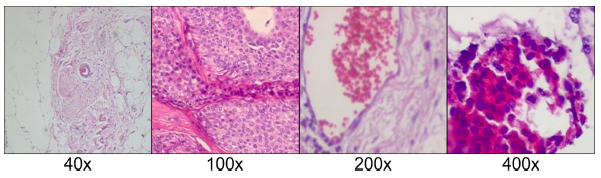
\includegraphics[scale=1]{figures/breast_histoimg_multiple_scales.png}}
	\caption{Example of histological images, captured at multiple magnification factors. Image from \cite{bayramoglu2016deep}}
	\label{histo_img}
\end{figure}

Due to the characteristics of these images, annotation in this field remains extremely expensive. Even a single sample requires many work hours from a trained expert, usually a doctor. Although not as costly as annotation, diagnosis also requires notable effort thus automating this process through the use of intelligent methods has the potential to streamline a process which affect millions of patients and non-patients. 

Fully automated systems in this field would allow people to get regular checks at a low price. This is essential in combating diseases like cancer in which early diagnosis drastically increases the survival rate. The promise of such a model encouraged researchers to develop various datasets focused on different organs and their organs including: liver, prostate, colon and breasts.

One class of Deep Learning models which recently obtained impressive results in multiple histopathology Computer-aided Diagnosis problems are \textbf{Multi-task (MT)} models. The benefits of the Multi-task Learning \textbf{(MTL)} paradigm \cite{caruana1997multitask} are manifold. First of all, this type of approach usually results in algorithms with better generalization. Secondly, as a single sample may be used for two predictions, some components of the network, such as encoders, are able to exploit this increased data efficiency and achieve faster model convergence. Moreover, training a single Multi-task network requires less computational resources when compared with the prospect of training two independent networks. 

All these desirable qualities make Multi-task models well suited for intelligent applications in Medicine, especially in Digital Histopathology where sample scarcity and massive image dimensions encourages the maximization of data efficiency and the reduction of the computational cost. 

The aim of this work is to analyse recent approaches from the Digital Histopathology field which employ Deep Multi-task models and identify possible future research directions. The rest of this report is structured in the following manner. In \textbf{Chapter \ref{chapter:RelatedWork}} Deep Multi-task models are introduced. Next, \textbf{Chapter \ref{chapter:InvestigatedApproach}} analyses recent MT approaches applied in various histopathology problems. The advantages and limitations of the previously mentioned methods are discussed in \textbf{Chapter \ref{chapter:Discussion}}. Lastly, \textbf{Chapter \ref{chapter:5-Conclusions}} concludes the report.
\chapter{Background}
\label{chapter:RelatedWork}

Multi-task models are network architectures created with the purposes of solving multiple different but related problems in the same time. This approach yielded impressive results in many Artificial Intelligence subfields such as: Computer Vision, Natural Language Processing and Reinforcement Learning as shown in \cite{crawshaw2020multi}.

Training a model using Multi-task Learning can result in numerous benefits including faster inference and training, when compared to two or more separate networks; reduced overfitting and information optimization, as each sample becomes more valuable in a MTL environment. On the other hand, the cost of all these advantages comes in the form of the increased complexity of finding symbiotic tasks. In some scenarios, stabilizing the MT network can become a cumbersome task. This is known in the literature as \textit{negative transfer}, an unfortunate case in which learning valuable information in one task hinders the performance of one or all other tasks encapsulated in the model.

Carefully choosing tasks and formulating them in a way which benefits each other is not an exact science, which follows certain protocols, at least yet. At the moment this combination is done based on intuition and through experimentation thus reducing the negative transfer can be seen as "the art" of Multi-task models. 

There are multiple works in the literature which showcase the unreasonable effectiveness of Multi-task models, where multiple tasks "cooperate" to improve the performance in all problems tackled by the multi-headed network. Besides the increase in performance, MT has another interesting quality namely the fact that it more closely reflects human reasoning. The human learning process is almost never done in isolation, any new concept is learned through the prism of previous experiences and knowledge. Additionally, when learning multiple new concepts in the same time, the human mind usually attempts to find relationships between them. 

All this being said, the combination of multiple tasks can be achieved through multiple categories of MT architectures identified in works such as \cite{crawshaw2020multi} and \cite{zhao2023multi}. The most prevalent are the following three: cascaded, normal (parallel) and cross-talk (interactive). A schematic illustration of these can be seen in \textbf{Figure \ref{mt_net_categ}}.

\begin{figure}[htb]
    \centering
	\centerline{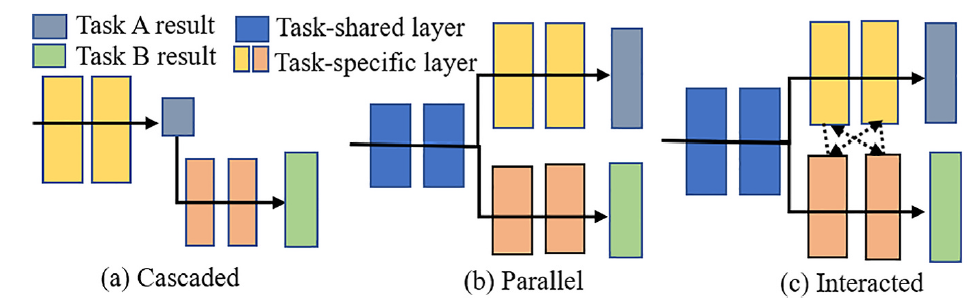
\includegraphics[scale=0.8]{figures/categories_mt_nets.png}}
	\caption{Examples of Multi-task networks classes: (a) cascaded (b) normal / parallel (c) cross-talk / interactive. Partially taken from \cite{zhao2023multi}.}
	\label{mt_net_categ}
\end{figure}

The most ubiquitous Multi-task type of network is the parallel one. In this design, a common encoder extracts valuable features which are sent in multiple independent task specific modules. Depending on the relation between the approached tasks the individual modules can be further connected via one or multiple fusion blocks in  order to further increase performance, resulting in a interacted or cross-task MT model. A cascade network is obtained when the result of one task is used as an input or feature for the remaining tasks.

Depending on the school of thought, some researchers argue that networks which process Multi-modal inputs are also included in the MT class of models. For the purposes of this report we will consider only approaches from the previously described three categories, although we will not disqualify multi-modal architectures as long as they are also part of said MT classes.

In \cite{zhao2023multi}, a vast number of medical applications of Deep Multi-task models are presented, briefly described and categorised based on their architecture and entity present in the input images. The authors showcase numerous approaches in which the MTL paradigm was used to improve performance in clinical practices which diagnose the following body areas and systems: brain, eyes, chest, cardiac, abdomen, musculoskeletal. Furthermore, they also offer a description of methods which processes histological images. 

This report differentiates itself from this impressive existing prior work through the following aspects:
\begin{itemize}
  \item The selection of papers.
  \item The perspective from which the analysis is conducted, as this report will focus on the choice of tasks (i.e. classification +  segmentation). 
  \item The granularity of the analysis especially for the papers considered to be the most representative in their category.
\end{itemize}
\chapter{Deep Multi-task Models for Histopathology}
\label{chapter:InvestigatedApproach}

We identified two different types of MT approaches in the field of Histopathology when it comes to the types of combined learning procedures. The more common one comes in the form of a MT network which learns through two or more supervised objectives. In the other class of approaches a supervised task is taught simultaneously with a self-supervised or even unsupervised one. The former is described in \textbf{Section \ref{hsmm}}, while \textbf{Section \ref{ssshmm}} present the latter class of intelligent algorithms.

\section{Fully Supervised
Multitask Models}
\label{hsmm}

We classify approaches which combine multiple supervised tasks based on nature of the combined objectives. Most MT networks perform two or more classification in the same time. These type of approaches will be presented in \textbf{Subsection \ref{classification_mt}}. In \textbf{Subsection \ref{classification_reg_mt}} we present a technique which combines a classification objective with a regression problem. We continue by describing intelligent techniques which perform multiple segmentation's simultaneously or a segmentation accompanied by another Image-to-Image inference in \textbf{Subsection \ref{segmentatiopn_mt}}. The last subsection from this section, \textbf{Subsection \ref{class_recog_mt}} analysis methods which fuse classification and segmentation. We decide to also include classification-detection hybrids in this part, as both segmentation and detection act as a localization and recognition tool.

\section{Multi-task Classification Models}
\label{classification_mt}
A pioneering work from the field  was introduced in \cite{bayramoglu2016deep}, where histological breast cancer images are classified as benign or malignant. This early MT approach, is also taught to predict the magnification factor. The resulting parallel architecture performs similarly to its single class equivalent showcasing that even early MT approaches allowed for the combination of multiple tasks without loss in performance. 

As deep learning matured, the performance of Multi-task models continued to improve. Early approaches including the previous one evolved from simple binary-classification between benign and malignant tissue to fine-grained multi-class classification of the cancer cells as is the case with the intelligent algorithm proposed in \cite{li2020multi}. Furthermore, their proposed parallel MT network also predicts the severity of breast cancer through the other classification head which classifies the tissue's grade in one of three classes. For the first objective, this method was able to achieve state-of-the-art results reaching a test accuracy of around 93.43\%.

One limitation in the Digital Pathology space when compared with other areas in which AI showed impressive results is the lack of large, medical datasets which would allow \textbf{Transfer Learning (TL)}. Pre-training on ImageNet \cite{deng2009imagenet} allows networks to learn many valuable features for many other classification problems. The sheer size of it also made the dataset the choice even in the medical field, although it contains no medical image. In order to fill this gap in medical Computer-Vision, the authors of \cite{mormont2020multi} propose a Multi-task approach able to aggregate the information from almost 90,000 images from 22 datasets. A common encoder is connected to 22 task-specific fully-connected layers, each tasked with classifying images from one of the datasets resulting in another parallel MT architecture. The learning objective is to reduce the mean loss obtained by averaging all the individual task-specific loss functions. A scheme of the model can be observed in \textbf{Figure \ref{mt_pretaining}}. The authors experimented with two established network backbones: ResNet50 \cite{he2016deep} and DenseNet121 \cite{huang2017densely}. Between the two, the first one performs better and improves the results when compared to ImageNet pre-training in almost all scenarios. The most significant increase is achieved in bone marrow classification exceeding the pre-existing pre-training method by around 6\%.

\begin{figure}[htb]
    \centering
	\centerline{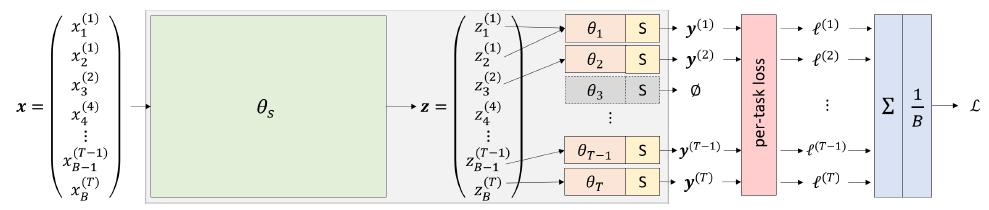
\includegraphics[scale=0.85]{figures/mt_pretraining.png}}
	\caption{The proposed MT arhitecture for pre-training on 22 datasets. Image from \cite{mormont2020multi}}
	\label{mt_pretaining}
\end{figure}

Recently, researchers employed multi-modal data in tandem with multi-task architecture in order to further develop the performance of existing approaches. One such approach was introduced in \cite{fan2022framework}. In this case, the multi-modality comes from the use of multi-parametric MRI images, a specific type of MRI which yields multiple types of medical data which better reflects the patient's state. The proposed network receives two inputs: the dynamic contrast-enhanced magnetic resonance images \textbf{(DCE-MRI)} and T2-weighted images \textbf{(T2WI}. Each has the benefit of better evidentiating complementary morphological characteristics of the human body. Starting from the ImageNet weights through the process of transfer learning, this multi-task network based of the VGG16 \cite{simonyan2014very} architecture learns to classify three cancer descriptors for breast cancer diagnosis: Luminal A, the histological grande and the Ki-67 expression. An illustration of the framework proposed in \cite{fan2022framework} is showcased in \textbf{Figure \ref{multimodal_multitask}}.

\begin{figure}[htb]
    \centering
	\centerline{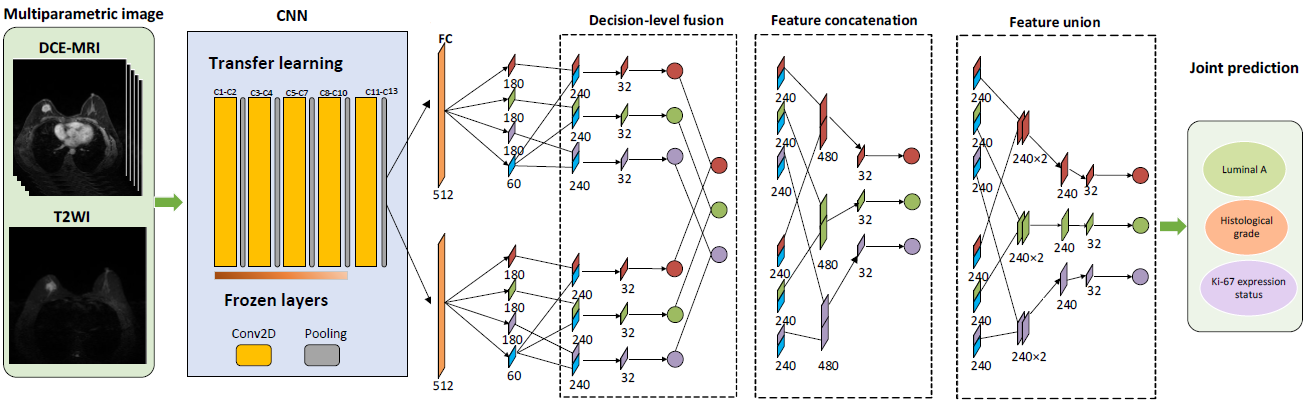
\includegraphics[scale=0.65]{figures/multimodal_multitask.png}}
	\caption{Multi-modal multi-task architecture for Luminal A, Histological Grade and Ki-67 expression status classification. Image adapted from from \cite{fan2022framework}}
	\label{multimodal_multitask}
\end{figure}

\section{Multi-task Model for Classification and Regression}
\label{classification_reg_mt}
Recently, researchers employed multi-modal data in tandem with Multi-task architecture in order to further develop the performance of existing approaches. One such approach was introduced in \cite{tan2022multi}. The proposed parallel Multi-task network receives two inputs: region of interests \textbf{(ROIs)} crops from a whole slide image \textbf{(WSI)} and mRNA expression data. The model dubbed, Multi-task
correlation learning \textbf{(MultiCoFusion)}, performs a classification task, in the form of cancer grade prediction in brain tissue and a regression task. The latter requires the network to predict the patient's survival risk. Unlike the previously described methods, MultiCoFusion does not have a single encoder. The multi-modality is processed through two different networks: ResNet152 for the histological images and a \textbf{Sparse Graph Neural Network (SGNN)} \cite{tan2021hierarchical} for the mRNA data. The extracted features are fused and passed to a Multi-task module which extract the most relevant features. Lastly one prediction heads is added for each task. Another unique aspect of this approach is the use of alternate learning instead of joint training, meaning that the network is updated based on only one objective for each batch. In this case, the determining objective is alternated after every batch.  An illustration of the proposed framework is showcased in \textbf{Figure \ref{multimodal_multitask2}}. MultiCoFusion is able to exceed all previous approaches, establishing itself as the state-of-the-art approach in both tasks.

\begin{figure}[htb]
    \centering
	\centerline{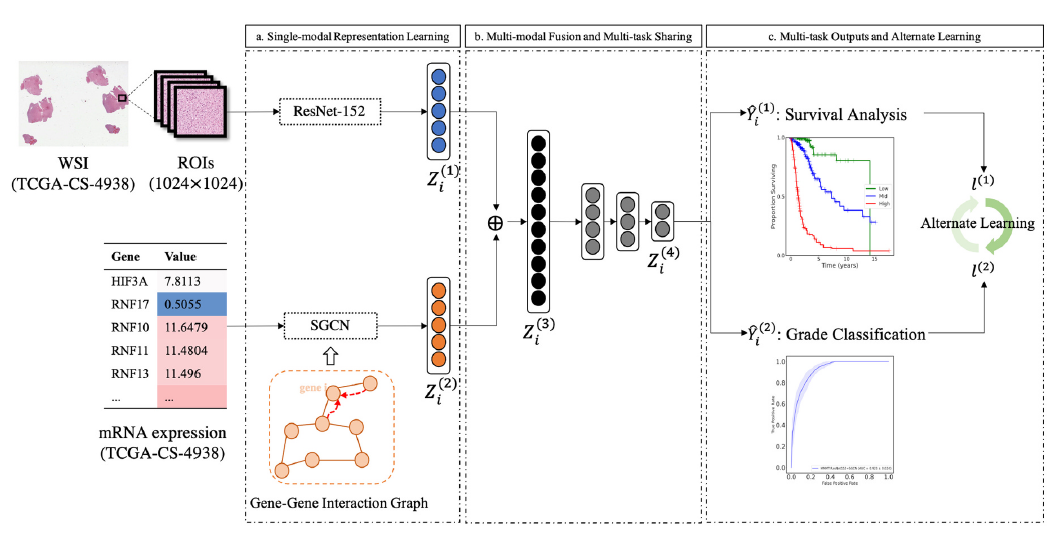
\includegraphics[scale=0.8]{figures/multimodal_multitask2.png}}
	\caption{MultiCoFusion architecture from \cite{tan2022multi}}
	\label{multimodal_multitask2}
\end{figure}

\section{Multi-task Segmentation Models}
\label{segmentatiopn_mt}

Another series of approaches combine two or more segmentation tasks in their MTL pipeline. Approaches \cite{wang2021bend} and \cite{rezazadeh2023multi} reformulate a single segmentation problem into a multi-objective one. The former approaches nuclei instance segmentation, while the latter tackles gland instance segmentation. In both problems, the entity instances overlap making a fine segmentation difficult resulting in a lower than desired performance. 

In both frameworks the instance segmentation is transformed in three segmentation objectives. Besides the original segmentation task, the researchers add adjacent objective which facilitate the separation of overlapping instances. In \cite{wang2021bend}, a nuclei distance map and the overlapping segmentation are performed in order to guide the main task. In \cite{rezazadeh2023multi}, the second segmentation head performs contour segmentation, while the third is tasked with overlapped gland segmentation, in a similar manner with the previous approach. 

The approach from \cite{wang2021bend}, named Bend-Net has an U-Net \cite{ronneberger2015u} structure with three decoders and gets its name from the novel proposed bending loss function. This objective is also proposed to deal with wrongly segmented overlapped nuclei. This is achieved by finding convex and concave points and the retrieved structures. Concave points are drastically penalized as they suggest the wrong merge of two independent entities. An example of how bending loss is computed can be observed in the following figure, \textbf{Figure \ref{bendingloss}}.

\begin{figure}[htb]
    \centering
	\centerline{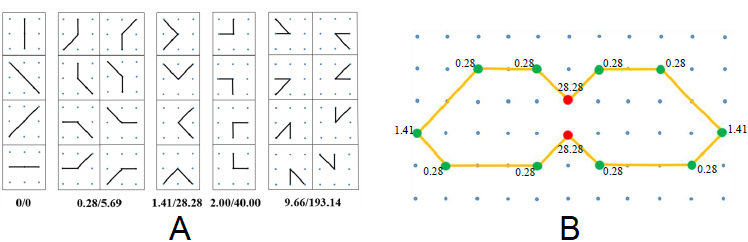
\includegraphics[scale=1]{figures/bend_loss.png}}
	\caption{(A) Examples of bending losses for different "curves". The same curve has a different score depending on wheter or not is seen as concave or convex. The values are presented as "convex score / concave score". (B) Example of bending loss computation for a given shape. \textcolor{forestgreen}{Green} indicates a convex point, whereas \textcolor{red}{red} indicates a concave point. Images from \cite{wang2021bend}. }
	\label{bendingloss}
\end{figure}

The Multi-task architecture combined with the bending loss outperforms numerous established networks in this task. Some results can be observed in \textbf{Figure \ref{bend_results}}

\begin{figure}[htb]
    \centering
	\centerline{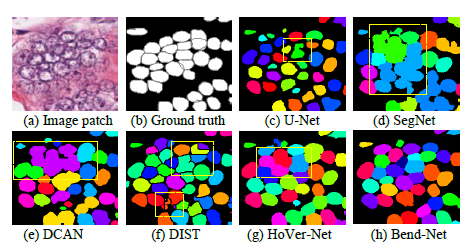
\includegraphics[scale=1]{figures/bend_results.png}}
	\caption{Inference example of nuclei instance segmentation for multiple neural networks. Image from \cite{wang2021bend}}
	\label{bend_results}
\end{figure}

In \cite{rezazadeh2023multi}, the authors demonstrate the effective of their proposed MT approach over the original starting point networks (DeepLabV3+ \cite{chen2018encoder} and U-Net). Through classic computer vision approach, starting from the instance segmentation ground-truth, they are able to obtain the contours segmentation map and the overlapping map, which in turn will be used as ground-truth in the MT pipeline. 

\begin{figure}[htb]
    \centering
	\centerline{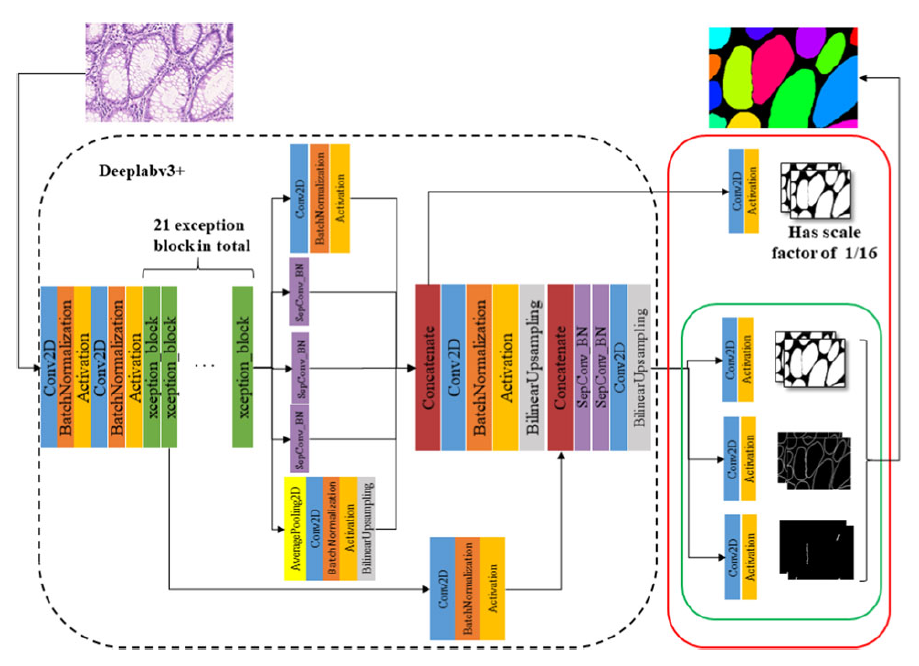
\includegraphics[scale=0.9]{figures/mt_deeplab.png}}
	\caption{Scheme of MT-DeepLab and MT-DeepLab-2 architectures from \cite{rezazadeh2023multi}. The black rounded rectangular encapsulated the DeepLabV3 network. The \textcolor{forestgreen}{green} area contains the MT-DeepLab components, while the \textcolor{red}{red} one also encapsulated the deeply-supervised MT-DeepLab-2 objective.}
	\label{mt_deeplab}
\end{figure}

The resulting network which performs the three segmentation tasks is simply named MT-DeepLab. As a way to continue the improvement of this model in the second version of the architecture, MT-DeepLab-2, a forth segmentation task is added. The model is encouraged to learn the segmentation map as soon as possible through the addition of this forth objectives which computes the instance segmentation loss at the start of the decoding path. Because the feature map has not yet gone through upsampling, this computation is done at a scale factor of 1/16. This type of learning is called Deep Supervision \cite{lee2015deeply}. Depending on the chosen metric either the first of the second MT-DeepLab outperform all other networks which were considered for the task of gland segmentation.

\section{Multi-task Models for Joint Classification and Recognition}
\label{class_recog_mt}

In \cite{yu2021large} a dataset for gastric cancer screening and localization is introduced. Furthermore, a MT network based on Deep Layer Aggregation is proposed \cite{yu2018deep}. Deformable convolutions \cite{dai2017deformable} are added to the model as many areas from WSIs contains little to no information, while other are densely packed with dense information. The method jointly learns to perform screening, a binary-classification problem in which tissue is classified as either normal or cancerous and semantic segmentation. The second task has the purpose of identifying the suspect areas in order to provide a justification for the diagnostic which could be verified by a doctor thus all cancerous cells have to be identified. 

\begin{figure}[htb]
    \centering
	\centerline{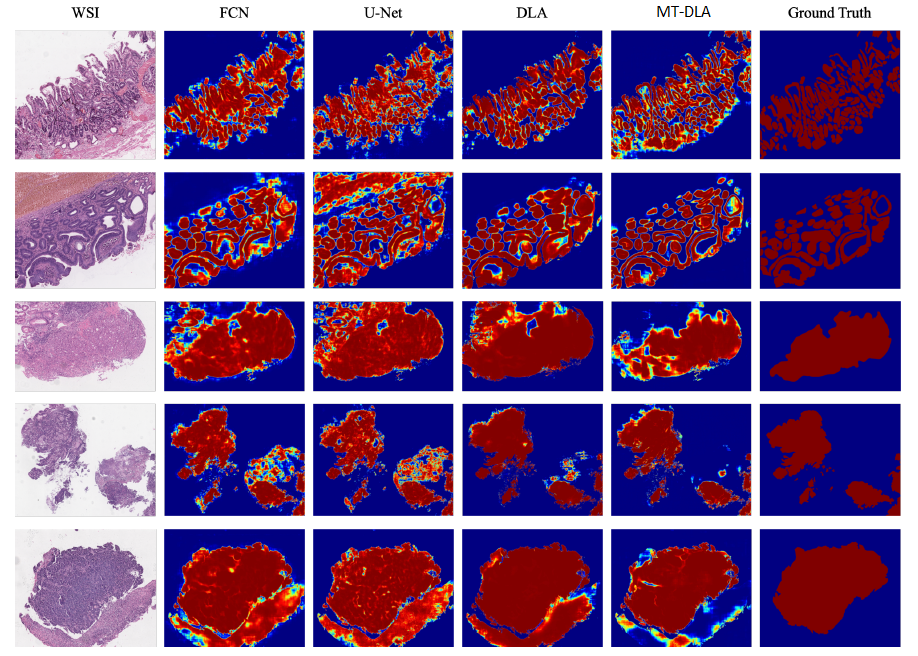
\includegraphics[scale=0.8]{figures/mtdla_results.png}}
	\caption{Predictions obtained by various networks for gastric cancer segmentation. Image from \cite{yu2021large}.}
	\label{mtdla_results}
\end{figure}

The proposed network, to which we will refer to as \textbf{Multi-Task Deep Layer Aggregation (MT-DLA)} achieves state-of-the-art results when compared with existing segmentation networks outperforming all candidates when it comes to both the segmentation and screening objective. The only metric in which the model is outperformed is specificity, which is not as relevant when it comes to identifying a dangerous disease in patients. Some results for the segmentation task can be seen in \textbf{Figure \ref{mtdla_results}}.

Paper \cite{dabass2022mtu} includes another Multi-task model which combines classification and segmentation, but unlike the previous approach it is applied for colon cancer. As many other networks which perform classification in a MTL environment in the field of Histopathology, the proposed network \textbf{Multi-Task U-Net (MTU)} classifies the tumour into either benign or malignant. Similar to the previous method, the segmentation is used to localize dangerous areas from the tissue. The design of this network is illustrated in \textbf{Figure \ref{mtu}}.

\begin{figure}[htb]
    \centering
	\centerline{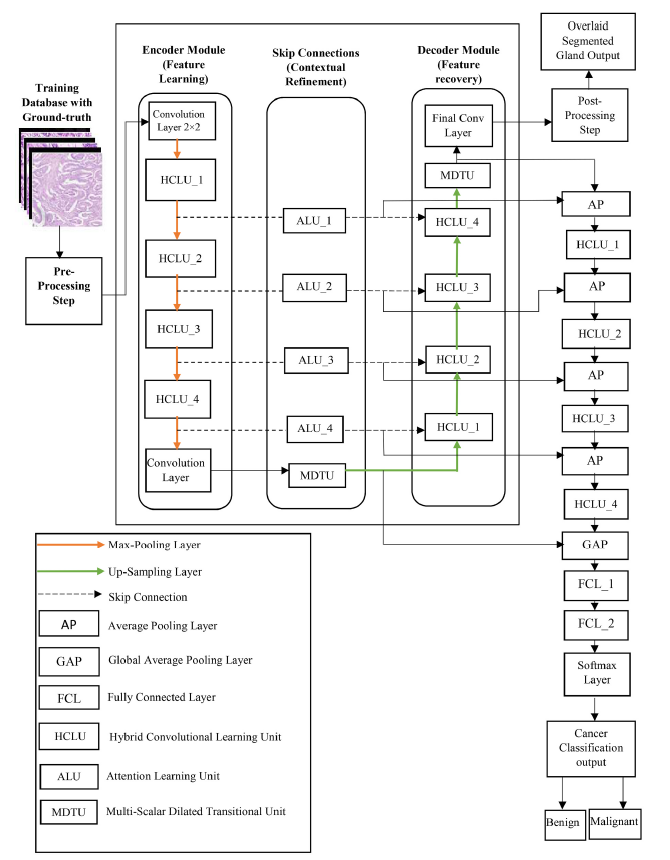
\includegraphics[scale=0.8]{figures/mtu.png}}
	\caption{MTU arhitecture diagram. Image from \cite{dabass2022mtu}}
	\label{mtu}
\end{figure}


Besides the addition of these additional objective, MTU also employs attention modules \cite{vaswani2017attention}. Another defining characteristic of the proposed approach is a novel block of layers design especially for WSIs, dubbed \textbf{Hybrid Convolutional Learning Unit (HCLU)}. The illustration of HCLU is showcased in \textbf{Figure \ref{hclu}}. This series of operations is a fusion between a Multi-Scalar Atrous Convolution, a Multi-Level Convolution and a Residual Block. The \textbf{Multi-Scalar Dilated Transitional Unit (MDTU)} is another newly introduced block which combines the results of four Atrous Convolutions with different dilation rates (1, 4, 8, 12). The features are aggregated through a \textbf{Global Average Pooling (GAP)} module. MTU was tested on two datasets, outperforming all its competitor.

\begin{figure}[htb]
    \centering
	\centerline{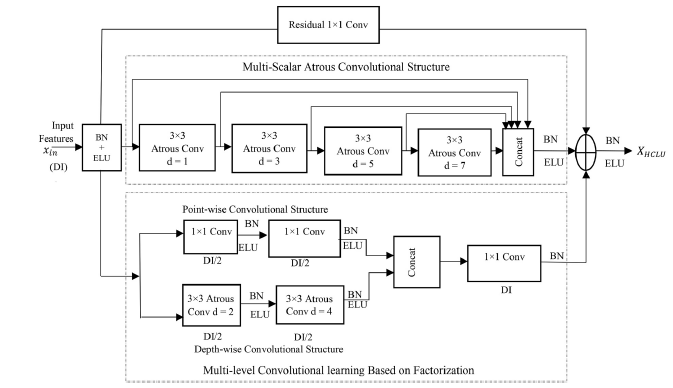
\includegraphics[scale=1]{figures/hclu.png}}
	\caption{HCLU block design. Image from \cite{dabass2022mtu}}
	\label{hclu}
\end{figure}

Similar to the work conducted in \cite{crawshaw2020multi}, paper \cite{graham2023one} introduces a MT network for processing different types of entities: nuclei, glands, tissue and lumen. The proposed model, named Cerberus. employs a common encoder which feeds data to three parallel decoders tasked with segmentation (nuclei, glands, lumen) and a module forth parallel module for tissue type classification. This allows the encoder, built following the structure of ResNet34, to learn rich features from multiple heterogeneous datasets, addressing data scarcity. U-Net like decoders are constructed for the segmentation tasks. The model achieves state-of-the-art-results exceeding the accuracy of other models in gland segmentation by almost 8\% and in lumen segmentation by around 10\%. An overview of the proposed framework is displayed in \textbf{Figure \ref{cerberus}}.

To further demonstrate the effectiveness of the encoder and their Multi-task learning strategy, the backbone is also used in two other transfer learning experiments. First of all, the pre-trained Cerberus encoder is used for the classification of nuclei. Next, the backbone is also employed in a detection task. Through the addition of object detection specific blocks which follow the RetinaNet \cite{lin2017focal} architecture, the model is able to learn to detect Signet ring cells. In nuclear classification, the pre-trained backbones yield a 4.6\% improvement on the test dataset when compared to previous approaches. It must be noted that in this experiments the pre-trained backbone is fully frozen.

Lastly, the authors tackle the of object subtyping. In this task, the segmented cell is further classified into four finer labels. As in the previous experiment the rest of the network is frozen, while the newly introduced decoder is taught to perform the multi-class segmentation. In all the experiments, Cerberus is shown to be a powerful network due to its encoder's ability to extract general, high-quality features.

\begin{figure}[htb]
    \centering
	\centerline{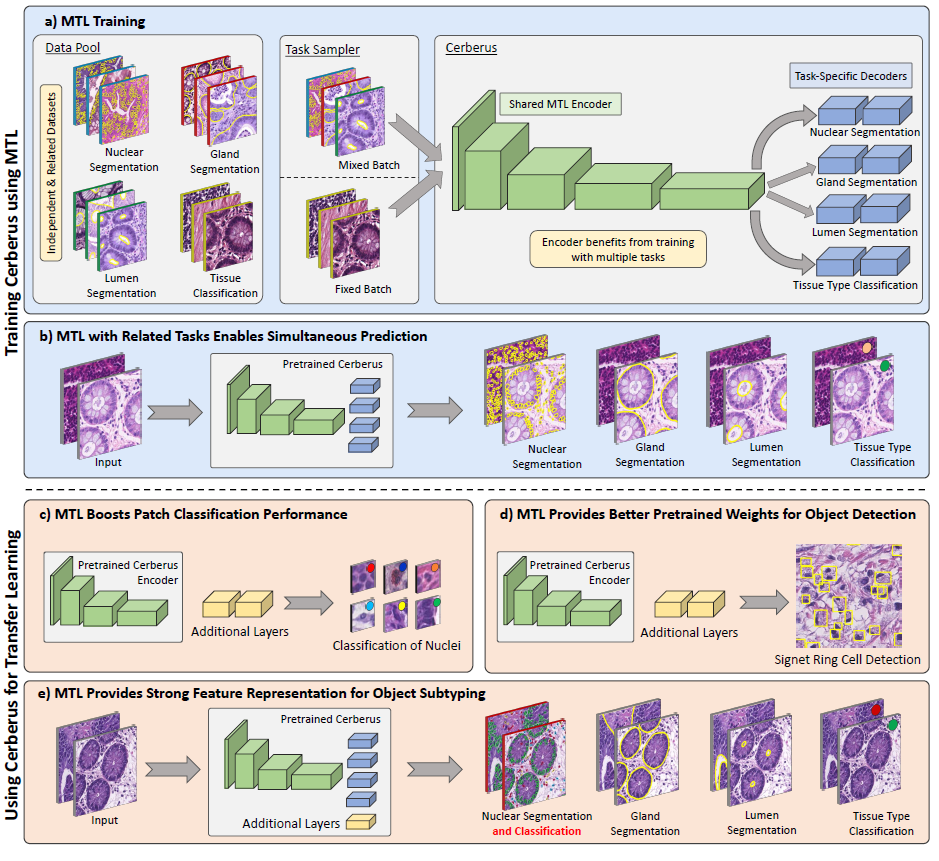
\includegraphics[scale=0.9]{figures/12.png}}
	\caption{Cerberus framework overview. Image from \cite{dabass2022mtu}}
	\label{cerberus}
\end{figure}

section{Supervised-Self-Supervised Hybrid Multitask Models}
label{ssshmm}

Reconstruction + Classification
cite{tellez2020extending}

Similarity + Image Reconstruction
cite{marik2022supervision}





\chapter{Discussion}
\label{chapter:Discussion}

Multi-task learning approaches have numerous benefits, many being especially useful in the field of Digital Histopathology. Training strategies which allow the encoder to learn from multiple datasets address limitations posed by data scarcity. This yields an increase in performance when compared to single-task models. Moreover, even in setting in which the MTL paradigm is not used to this end, the fusion of two symbiotic objectives results in impressive performances. The MT architecture can also be used to boost the accuracy even when a single problem is tackled by reformulating the problem into multiple objectives. This showcases the versatility of this technique. Lastly, as multi-modal network become more popular, MT networks establish themselves as a worthy candidate to process and mini information from heterogeneous data as prediction heads can be added for each data type as a way to complement the main objective. All these characteristics set MT models apart as a approach which can infer in a manner which is closer to human logic, having a lot of potential in the explainability area as the field further matures. 

On the other hand, the MT Histopathology literature is still in early phases. Most models compare themselves against general architectures, which were not tailored for the approached medical task. The desire to solve multiple problems in the same time, created a need for new datasets which contain annotation for all objectives. This is an extremely costly endeavour, which satisfied the requirements only in few cases. Even if multiple datasets exist in the field, combining them can prove to be cumbersome as the resulting super-set would have samples in which not all tasks have a ground-truth, as most databases only contain annotation for one or a few tasks. 

When it comes to the model themselves, the main limitation is the fact that almost all approaches follow the parallel MT architecture. Further experiments could be conducted in order to evaluate the possible improvements obtained through the transformation into a cross-talk or interactive approach. Vast studies could be conducted in order to search for effective fusion techniques between otherwise independent decoders, especially when two of the objectives are closely knit. 

Lastly, another underdeveloped niche which could prove to be a promising research direction consists of combining supervised objectives with semi-supervised or even unsupervised ones. This would alleviate the need of costly annotation, even if the initial results have little to no chance of being comparable to the potential of two fully supervised ones.
\chapter{Conclusions}
\label{chapter:5-Conclusions}

In conclusion, Multi-task Learning is a powerful and versatile learning strategy, which can be exploited in order to create effective encoders applicable in numerous tasks with no required change. The valuable features mined by this intelligent approach can be used to obtain multiple relevant medical information through a single model pass, reducing training and inference time. This paradigm which lead to impressive performance in multiple tasks is still in early phases, at least in the medical image analysis area, leaving space for future research directions which could investigate relevant areas which were not yet covered by the existing literature. It is our firm belief that the current state of MT networks warrants further study especially when it comes to  cross-talk techniques and possible fusions between supervised and semi-supervised or unsupervised objectives.  



\bibliographystyle{plain}
\bibliography{BibAll}

\end{document}

